\documentclass{article}

%\usepackage{amsmath}
\usepackage{graphicx}
%\usepackage{hyperref}
%\usepackage{listings}
%\lstset{
%numbers=left
%}
\usepackage{url}
\usepackage[top=1in, bottom=1.25in, left=1.25in, right=1.25in]{geometry}

\begin{document}

\title{CSE 222A Project Proposal \\
		Coflow Scheduling \\
		\large Group 6}
\author{Ruby Pai \and Amit Borase \and Sreejith Unnikrishnan \and Stas Mushits \and Ritvik Jaiswal}
\date{\today}
\maketitle

\section{Introduction} \label{introduction}

Data parallel cluster applications running on fast CPUs are limited by relatively slower network connections. The coflow abstraction for such applications was recently proposed in \cite{chowdhury2012coflow}, which argued that identifying the individual parallel data flows associated with an application as a ``coflow'' and applying application-aware scheduling would improve application performance. Subsequently, Varys, a coflow scheduler was published \cite{chowdhury2014varys}, followed by Aalo, which improves on Varys \cite{chowdhury2015aalo}. Varys is based on heuristics that draw on insights about characteristics of an optimal coflow scheduler that would allow scheduling for minimal coflow completion time (CCT) or to meet a deadline.

The Varys scheduler was shown to improve CCTs by up to 3.16 times on average, and to increase the number of coflows meeting deadlines by a factor of 2 \cite{chowdhury2014varys}. This is promising not only for application performance, but has implications for issues such as data center energy efficiency, as most of the power wasted in data centers is due to CPUs idling while waiting for the network. However, a significant barrier to usage of coflow schedulers like Varys or Aalo is that they require coflows to be explicitly identified by the programmer to the scheduler via an API. This poses problems in terms of legacy code, programmer burden, and finally, in cases in which the coflows that exist in an application may not be obvious or known. 

Therefore, in this project, we propose to examine coflow scheduling in two parts. First, we will replicate the results of \cite{chowdhury2014varys} using the same trace, which is available on \cite{website:coflow-repo} and extend the experiment to traces for different data parallel applications. Second, taking Varys as the established state-of-the-art in coflow scheduling (as the code for Aalo does not appear to be available yet) we will examine the impact of incomplete coflow identification on the scheduler. Examining the robustness of the current state-of-the-art scheduler to incomplete coflow labeling will inform whether automated algorithms for identifying coflows, using for example machine learning techniques, which cannot be expected to be 100\% accurate, are viable with current coflow scheduling techniques.

\section{Approach}

As mentioned Section \ref{introduction}, the proposed project consists of two parts. The first part is to validate results from published literature, extending the scheduling results to new workloads. By examining how the scheduler performs with less than 100\% coflow labeling, the second part takes the first step in considering how the published result (the Varys scheduler in particular and coflow schedulers in general) might work with automated coflow identification, which we argue is important for the reasons stated in Section \ref{introduction}.

\section{Related Work}

So far, we have focused on the seminal work of Chowdhury et al on coflows and coflow scheduling \cite{chowdhury2012coflow, chowdhury2014varys, chowdhury2015aalo}. Though Aalo is the more recent result and the authors argue its overall merits over Varys, the code does not appear to be publically available (we have not contacted the authors). We thus focus on Varys, with a experimental setup that should be easily exendtible to Aalo, as both schedulers are implemented in Scala and expected to work with the coflow simulation code in \cite{website:coflow-repo}. Other work on coflow scheduling includes \cite{zhao2015rapier}, which integrates routing for a performance improvement, as well as other works cited in Section 9 of the August 2015 Aalo paper \cite{chowdhury2015aalo}. 

Since our primary interest is ultimately in examining the performance of coflow scheduling with less than 100\% labeling of coflows, we chose to use Varys, which is authored by the inventors of the coflow concept and for which the code is available. However, since Varys is based on heuristics, it is not currently clear to us what impact this has on the result for all possible coflow schedulers.

We are not currently aware of other work that performs validation of the Varys result and examines the performance of Varys with unidentified coflows, but plan further reading on coflow identification to continue searching for such. 

\section{Plan}

First, we will set up a cluster simulation environment. We anticipate obtaining 10 virtual machines via class resources. We are using Mininet \cite{website:mininet}, a network emulator that can create arbitrary topologies of hosts, switches, controllers and links, to set up a virtual cluster environment of about 100 hosts, along the lines of Figure \ref{fig:cluster_topology}. 

\begin{figure}[h]
	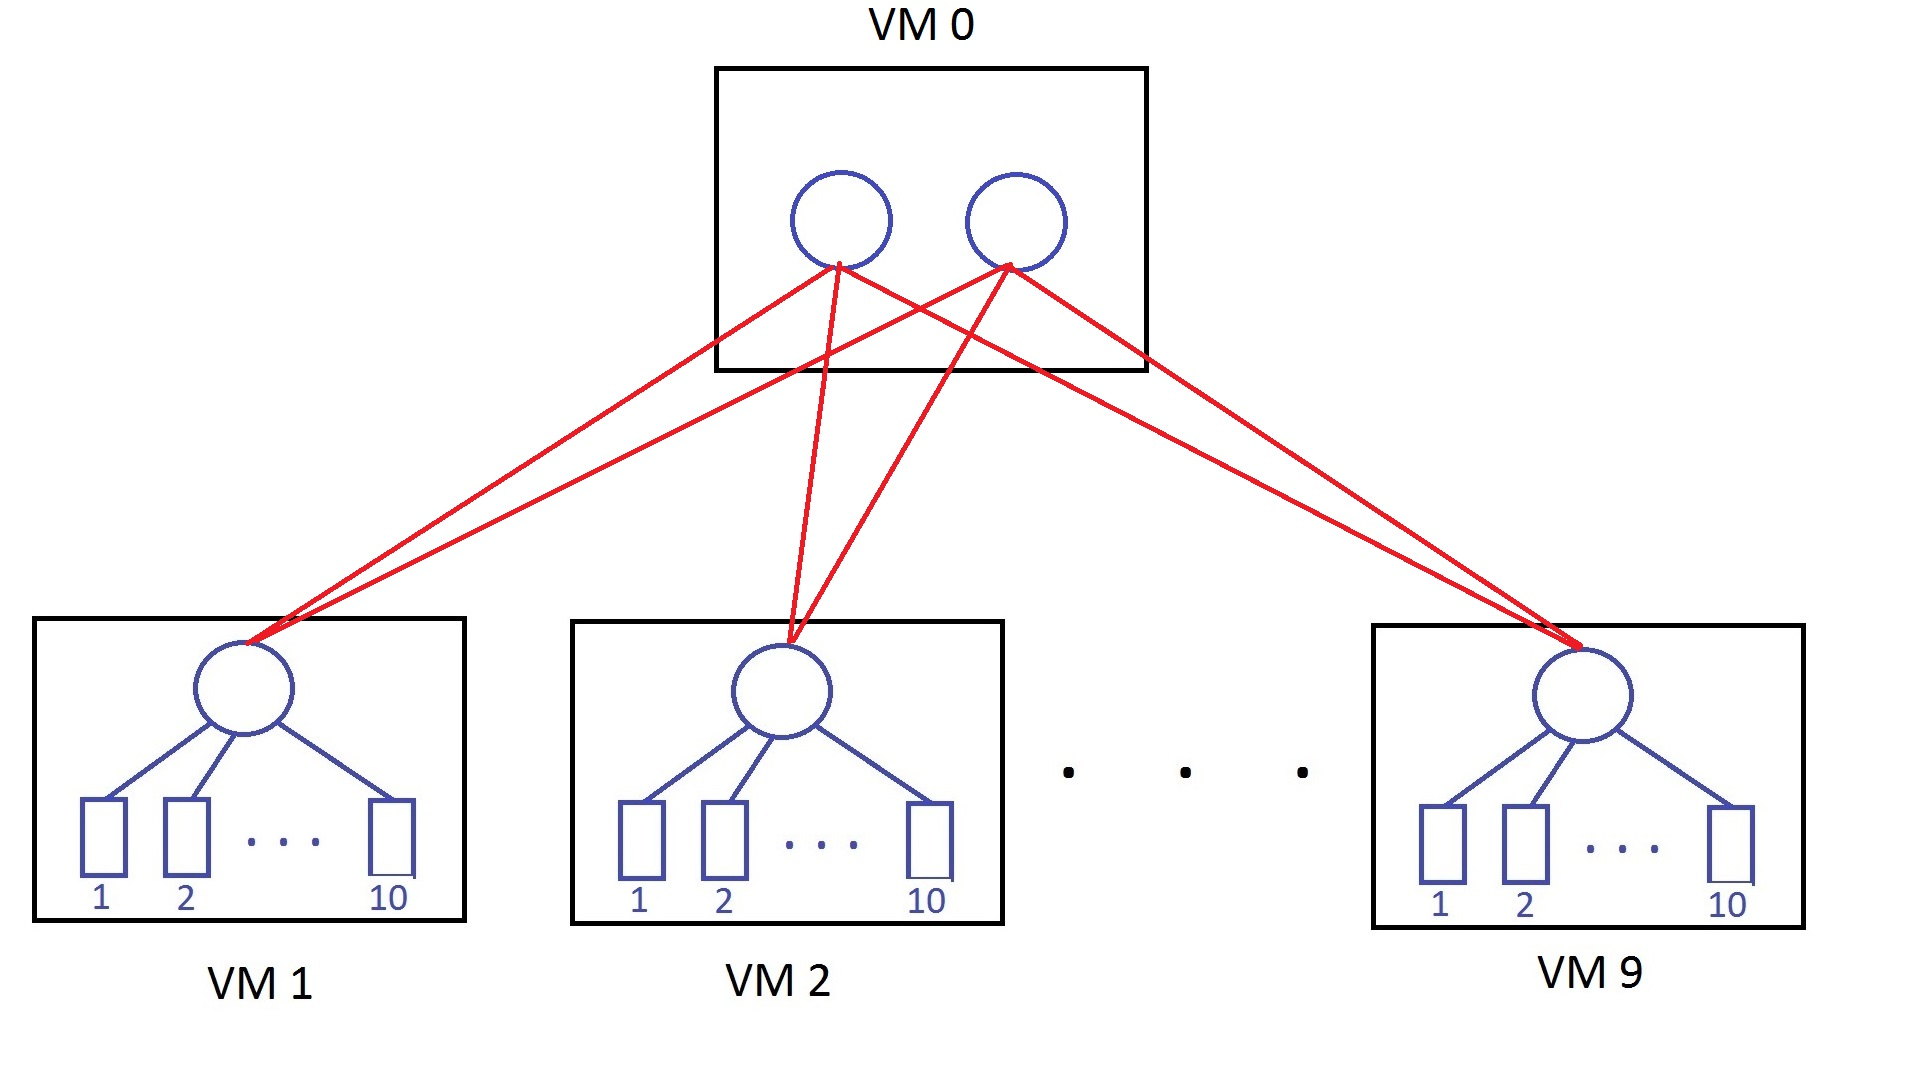
\includegraphics[height = 3in]{proposed_cluster_topology_final.jpg}
	\caption{Proposed topology for simulated cluster. Virtual machines are in black; mininet elements are in blue. We are looking into how to implement the inter-VM links in red. The simulation is thus the blue and red elements of switches, hosts and links.}
    \label{fig:cluster_topology}
\end{figure}

We are still trying to figure out how to implement the inter-VM links in red; GRE tunnels require distinct (source, destination)-tuples, so the two switches in VM 0 would be a problem. Alternatives using GRE would be either to just have a single high level switch, or to implement our entire simulation within one VM. A large number of network elements can be created on a single machine with Mininet, but while we have set up the indivdual VM building blocks to create Figure \ref{fig:cluster_topology} on the one VM we currently have, we have not examined whether implementing the entire cluster within one VM would work for our purposes. Until we obtain the additional VMs, we will work with a smaller topology within a single VM, which we have set up. 

Whatever the final setup selected, data rate must be selected appropriately to ensure that virtualization does not impact our experiment results, and testing performed to verify the correctness of our setup. Also, the scheduler performance metrics were coflow completion time (CCT) and number of coflows meeting their deadline over a per-flow scheduler. We need think carefully about the evaluation of these metrics in our experimental setup.

\section{Schedule}

By each of the given milestones, we plan to complete the following tasks.

1. Milestones 11/5 (2 weeks)
Complete evaluation with the trace available on \cite{website:coflow-repo}. We anticipate that once this is done, significant hurdles will have been cleared.

2. Milestone 11/24 (2.5 weeks)
Complete evaluation with other traces (11/5, one week). The significant work involved here is gathering other traces and adjusting them to our virtual environment. Also, we will be able to run the simulation without all coflows identified (11/24, one a half weeks). 

3. Deliverable 12/8 Poster and Final Report (2 weeks)

We will complete all experiments with less than 100\% coflow labelling and evaluate scheduler performance.

%\begin{thebibliography}{9}
%
%\bibitem{varys2014}
%Chowdhury et al
%Varys scheduler paper title.
%
%\end{thebibliography}

\bibliographystyle{plain}
\bibliography{coflow}

\end{document}
 
